\chapter{Direct multi-bed dynamic reconstruction: Supplementary material}
\label{chap:AppendixC}

Supplementary graphs, used in the analysis of the evaluated IsotoPK studies of chapter~\ref{Chap3_3:IsotoPK}, are provided here. Additionally, an brief simulation study for the behaviour of the spectral analysis model in the liver and the effects from the dual-input function is included.s

\section{Supplementary graphs}

\begin{figure} [h!]
\centering
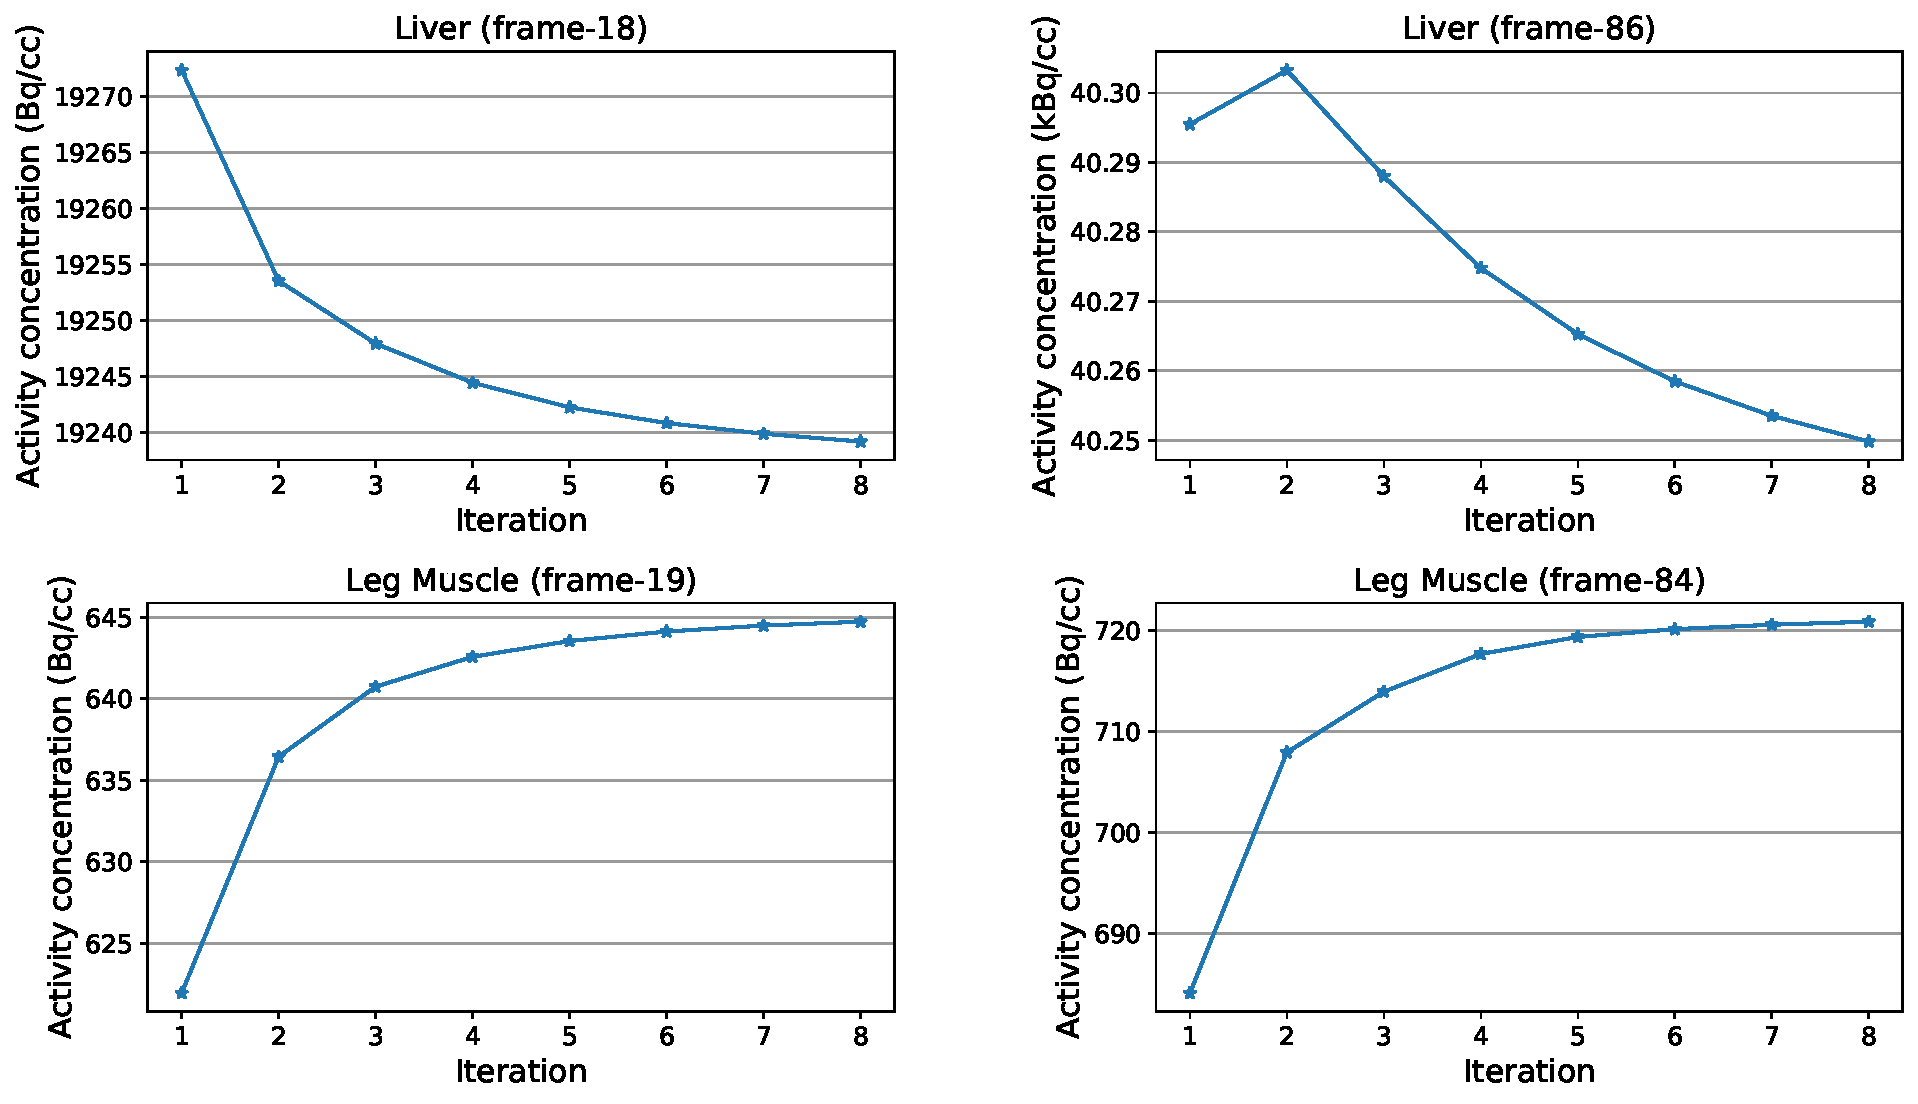
\includegraphics[scale=0.5,angle=0]{3_Results/3_3_DWB_Reconstruction/figures/3_3_IsotoPK_CTRL_DWB_3D_Convergence.pdf}
\caption{Liver (top) and Muscle (bottom) VOI mean versus iteration curves for 3D reconstruction. Shown for early (left) and late (right) frames of the \textit{CTRL} DWB acquisition including the DSB phase.}
\label{fig_3_3:IsotoPK_CTRL_DWB_4D_Convergence}
\end{figure} 

\begin{figure} [h!]
\centering
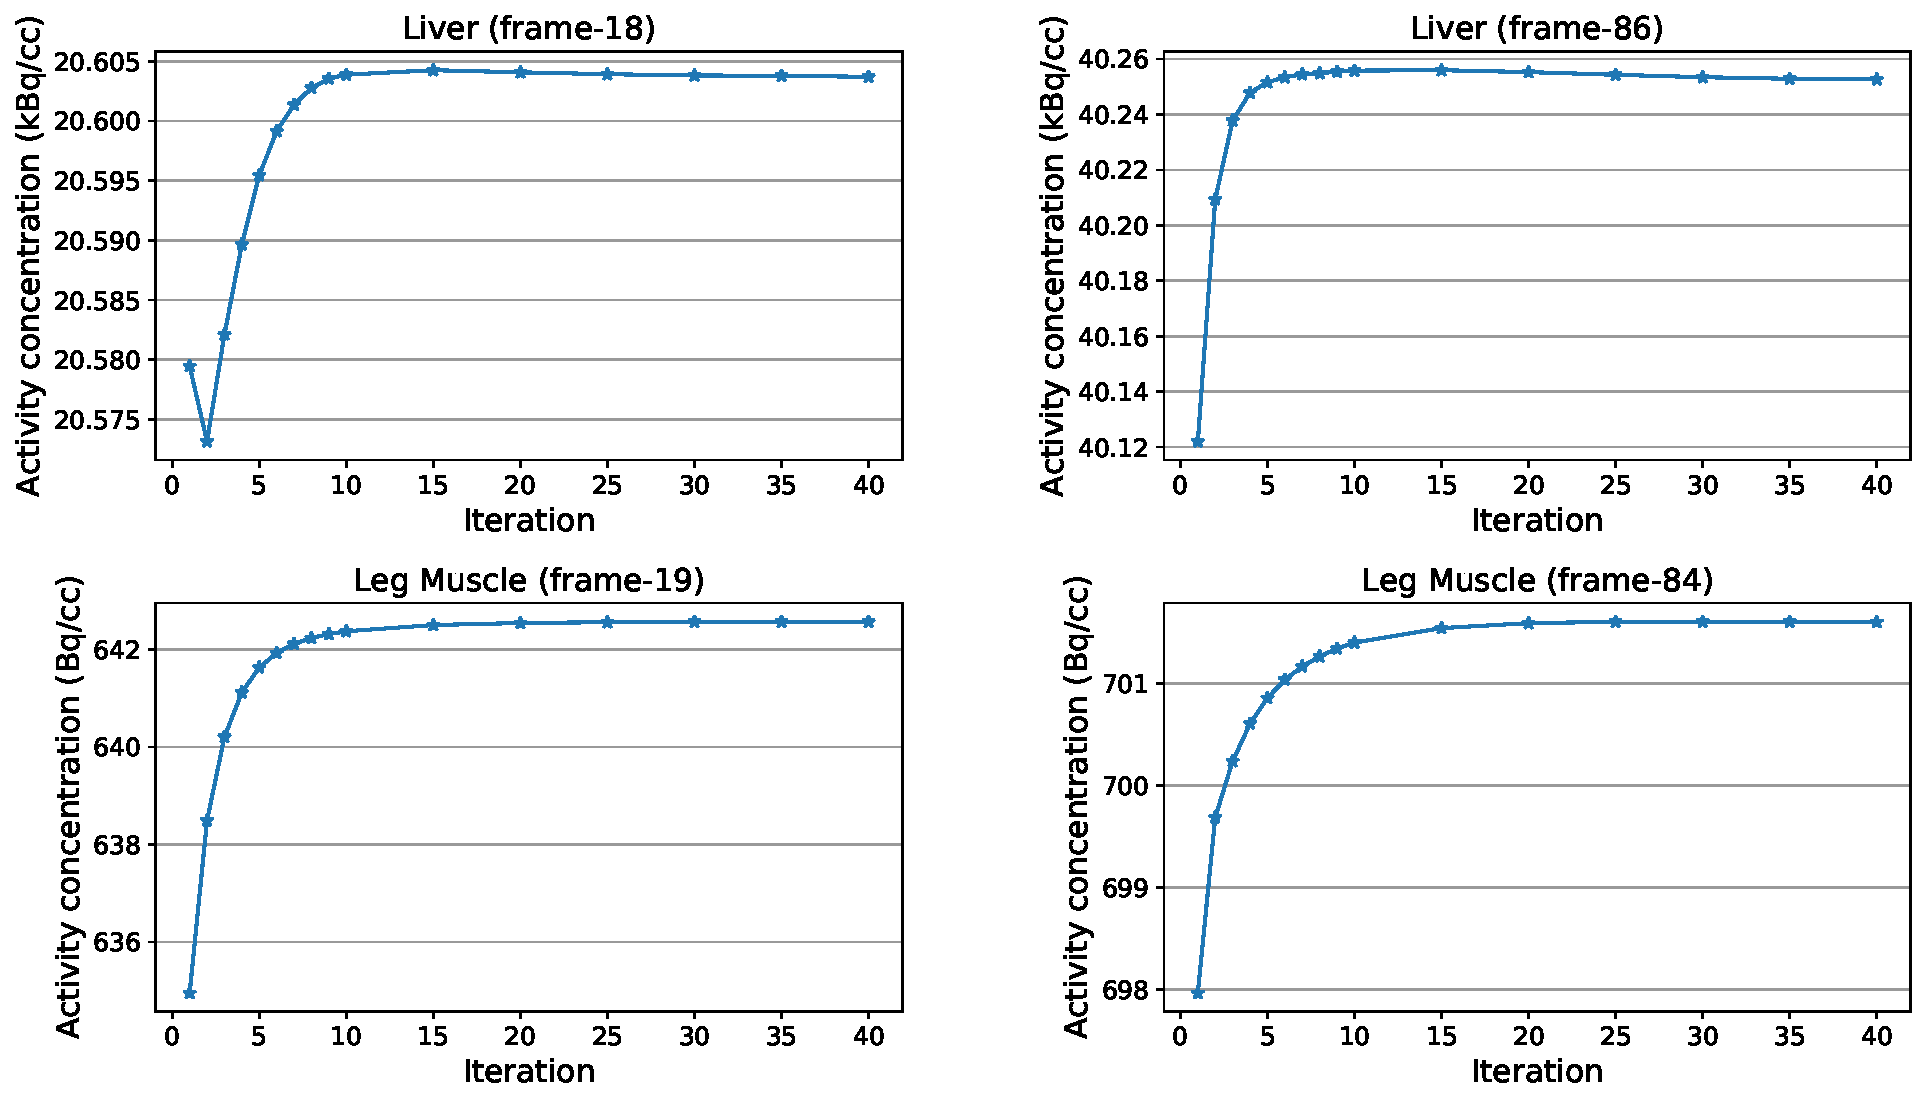
\includegraphics[scale=0.5,angle=0]{3_Results/3_3_DWB_Reconstruction/figures/3_3_IsotoPK_CTRL_DWB_4D_Convergence.pdf}
\caption{Liver (top) and Muscle (bottom) VOI mean versus iteration curves for 4D spectral reconstruction. Shown for early (left) and late (right) frames of the \textit{CTRL} DWB acquisition including the DSB phase.}
\label{fig_3_3:IsotoPK_CTRL_DSB_3D_Convergence}
\end{figure} 


\begin{figure} [h!]
\centering
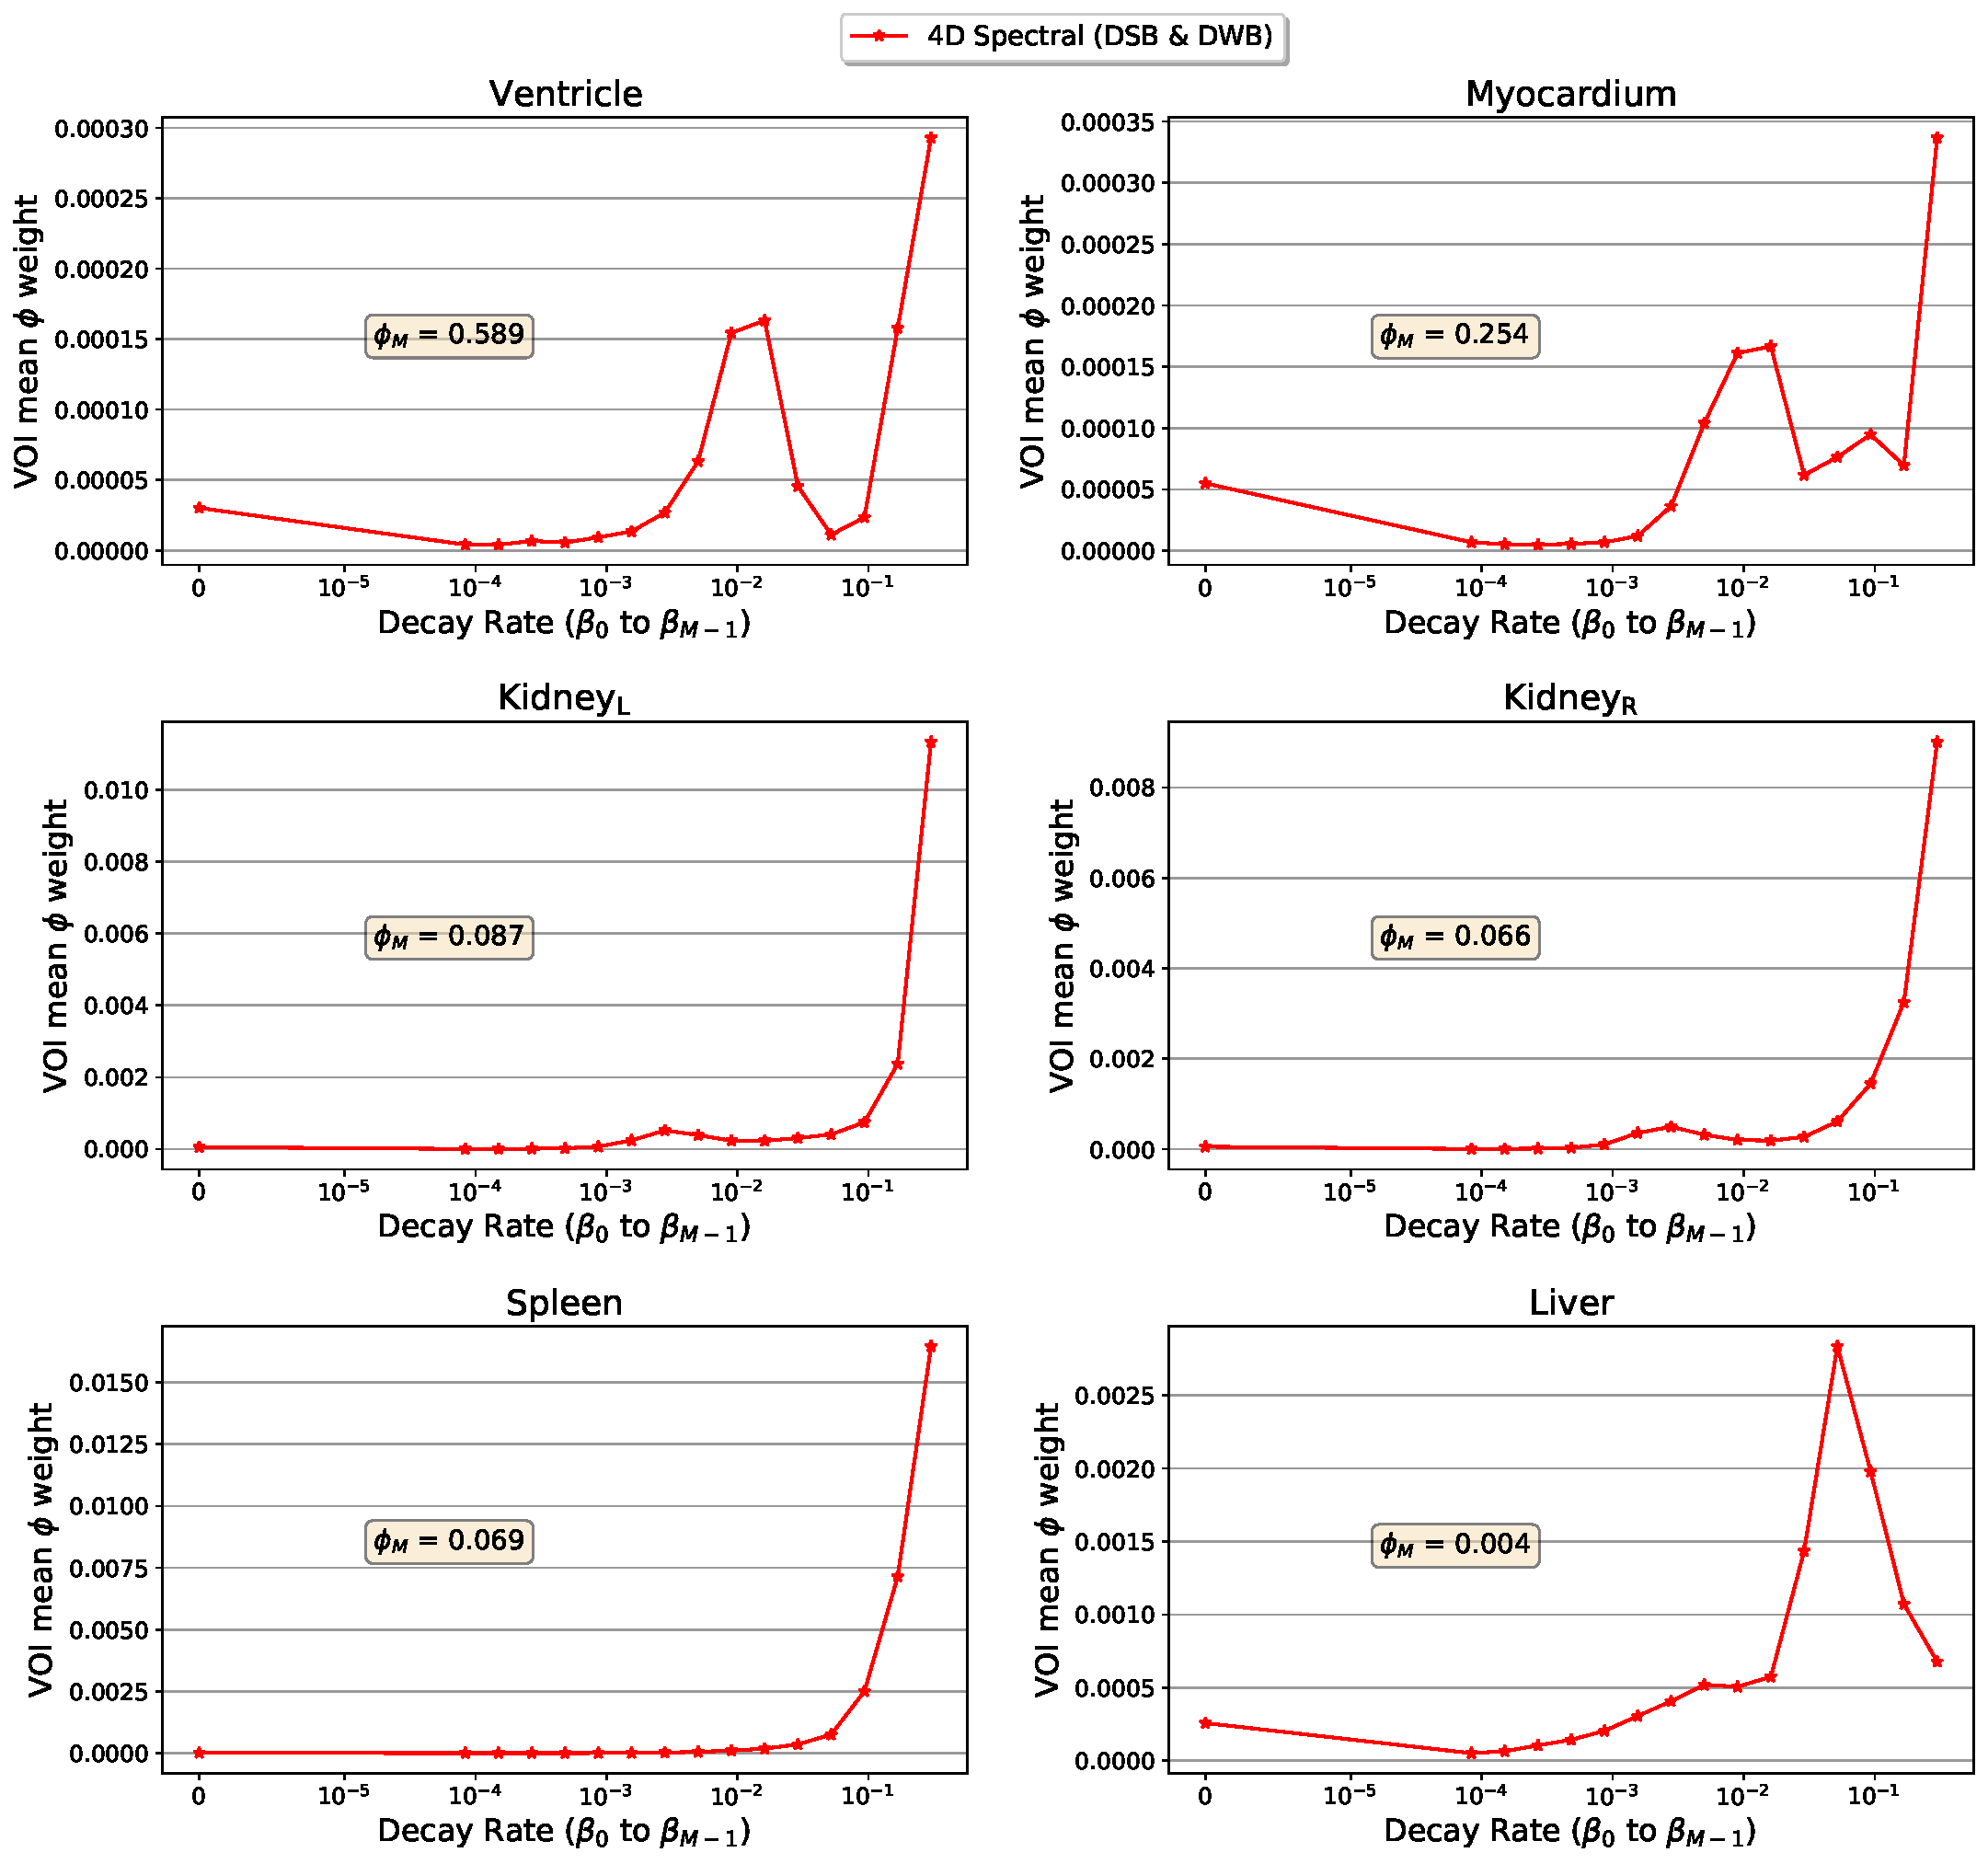
\includegraphics[scale=0.48,angle=0]{3_Results/3_3_DWB_Reconstruction/figures/3_3_IsotoPK_CTRL_DWB_SpectralParams_central_.pdf}
\caption{Spectral model coefficients average in VOIs.}
\label{fig_3_3:IsotoPK_CTRL_DWB_Spectrals}
\end{figure} 

\begin{figure} [h!]
\centering
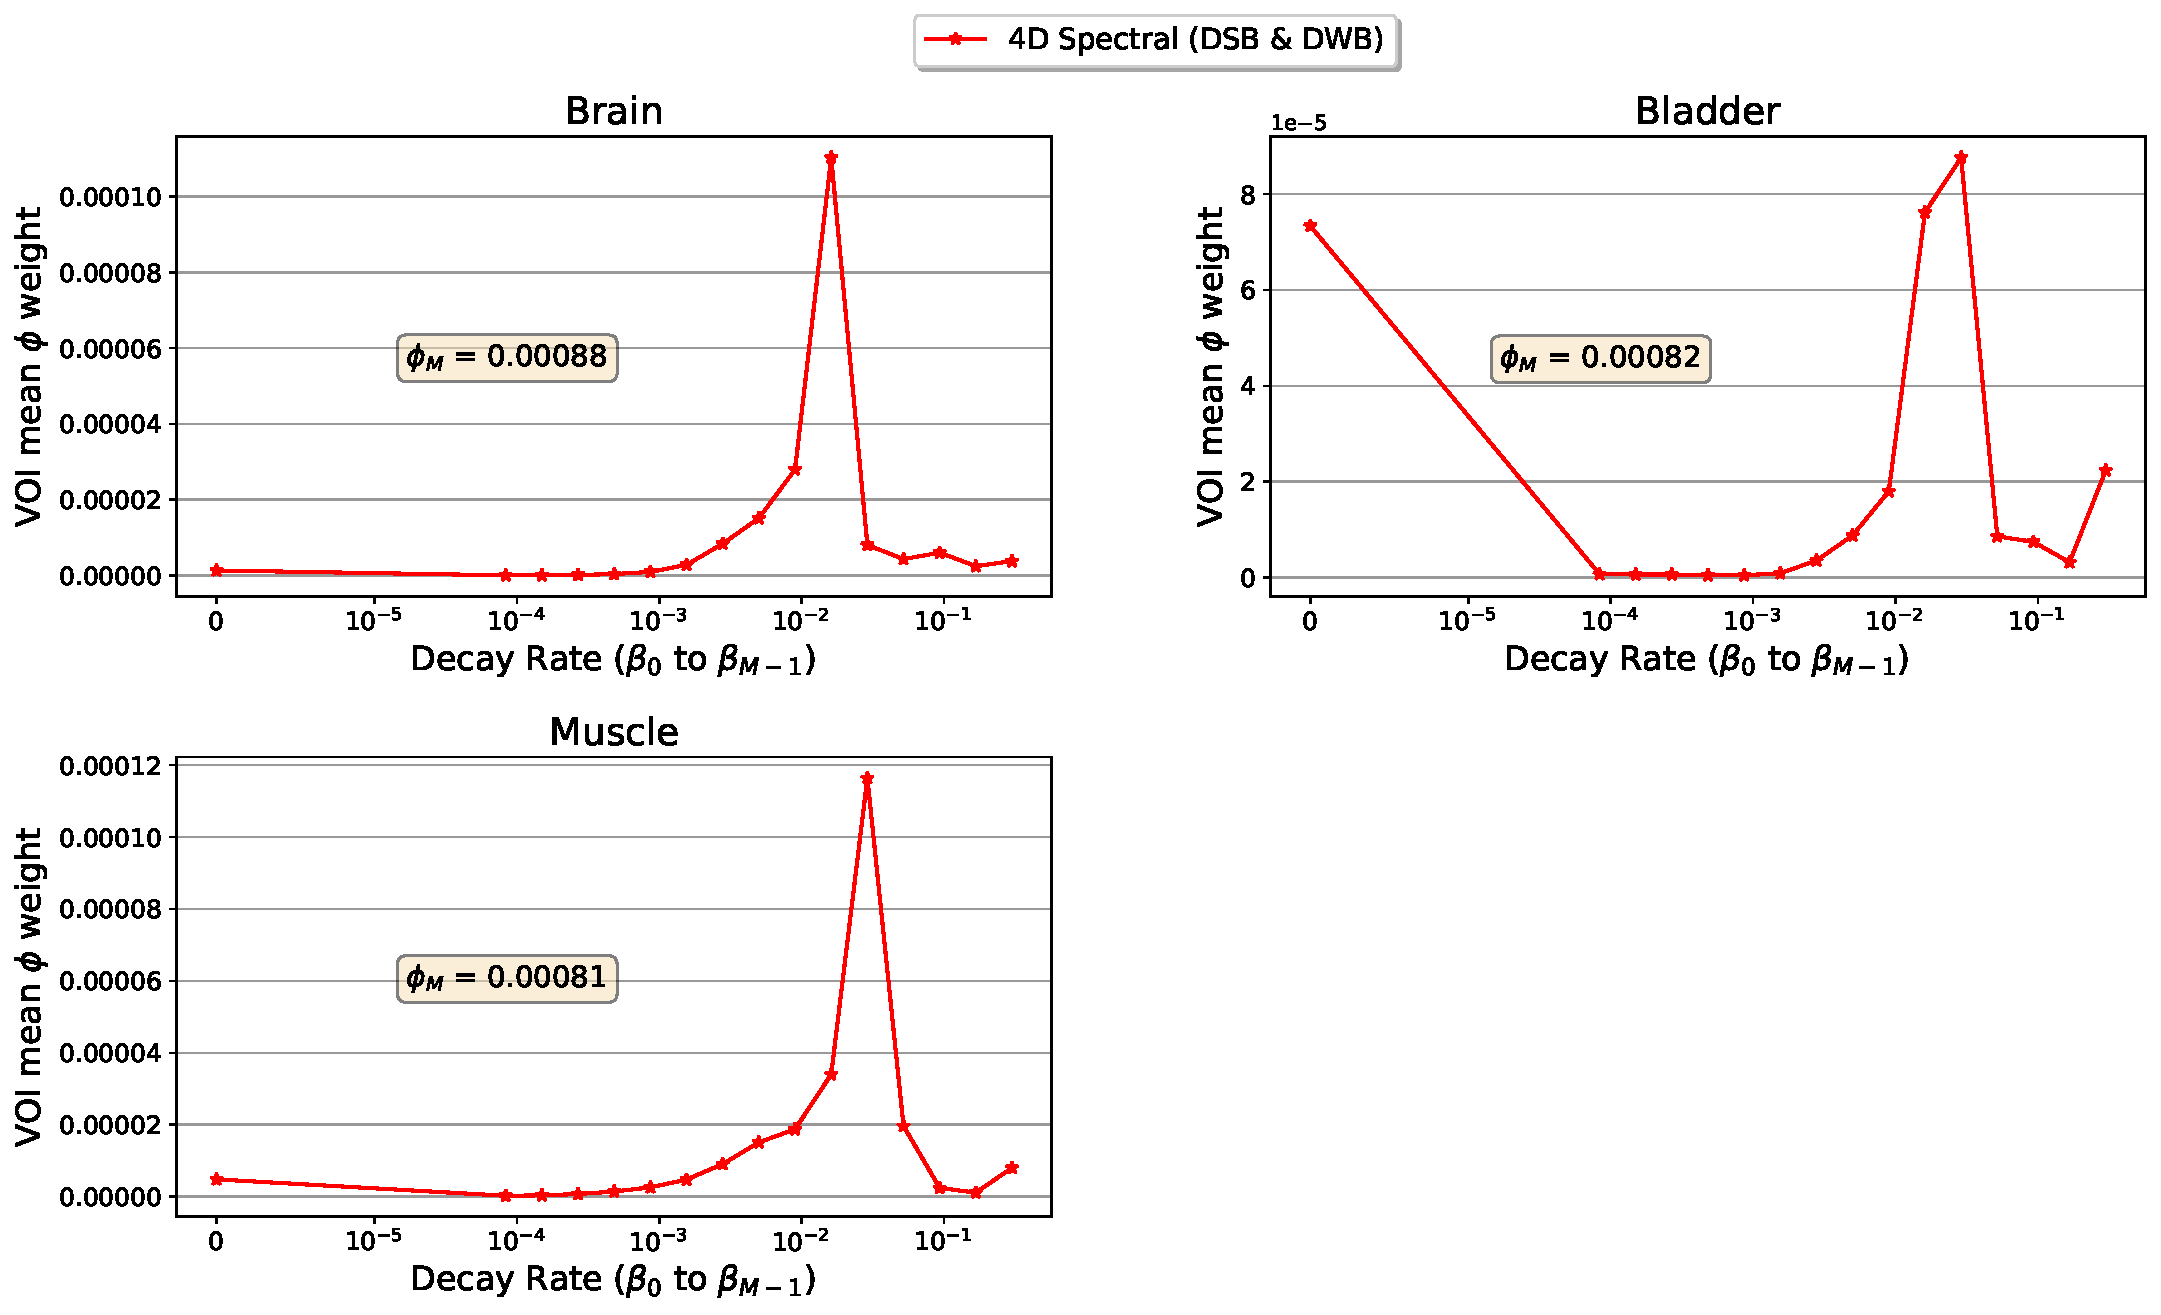
\includegraphics[scale=0.48,angle=0]{3_Results/3_3_DWB_Reconstruction/figures/3_3_IsotoPK_CTRL_DWB_SpectralParams_peripheral_.pdf}
\caption{Spectral model coefficients average in VOIs.}
\label{fig_3_3:IsotoPK_CTRL_DSB_Spectrals}
\end{figure} 

\clearpage
\section{Liver dual-input sim study}

\begin{figure}[h!]
\centering
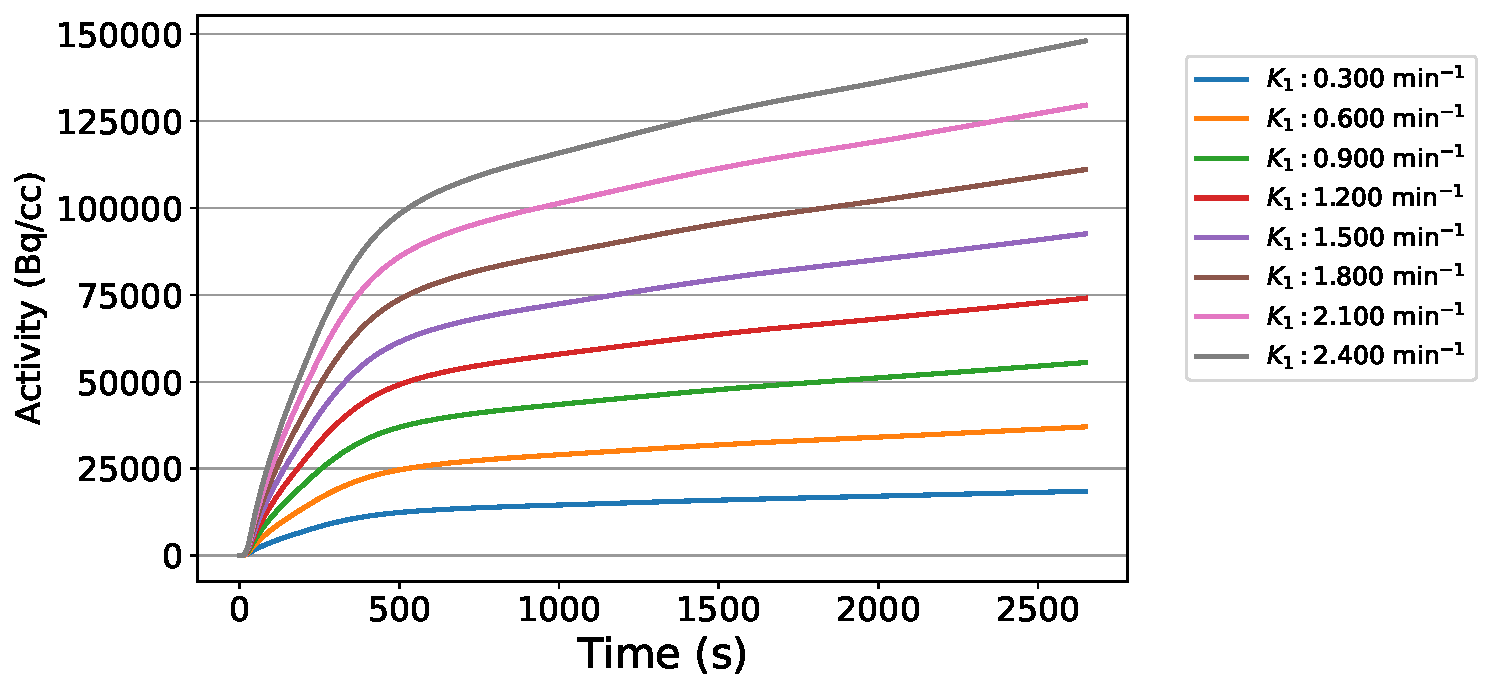
\includegraphics[scale=0.48,angle=0]{appendices/figures/ApendixC_multiple_K1.pdf}
\caption{Simulation of Liver TACs, using dual input function model and varying $K_1$ values}
\label{fig_3_3:K1_Sims}
\end{figure} 

\begin{figure}[h!]
\centering
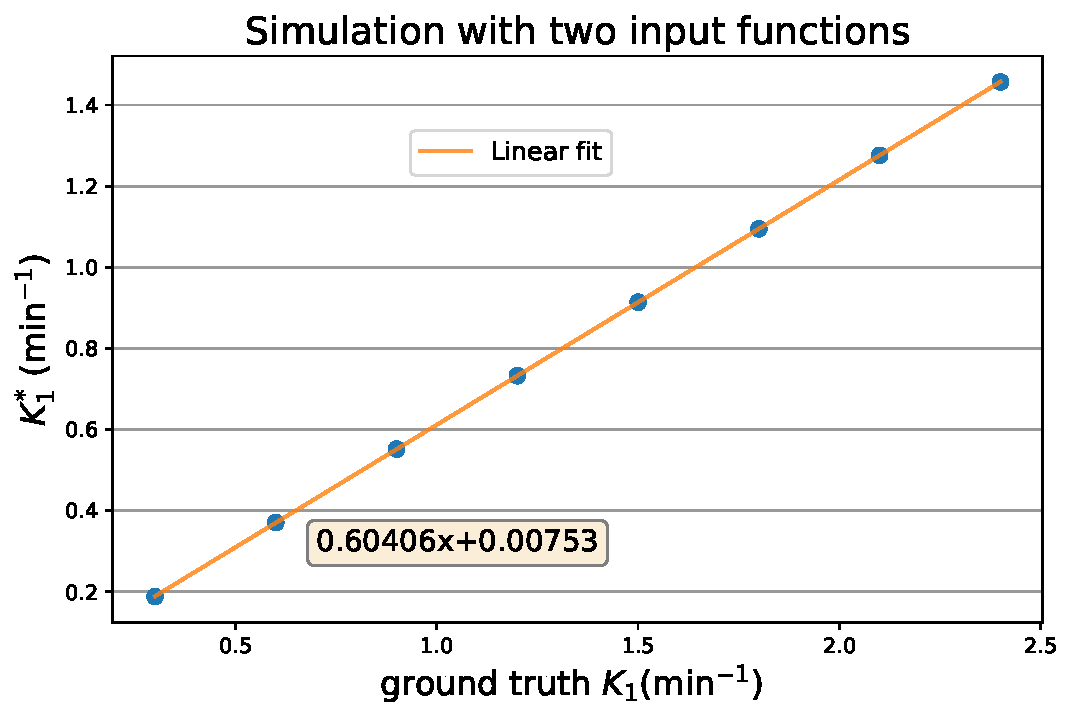
\includegraphics[scale=0.48,angle=0]{appendices/figures/ApendixC_multiple_K1_solution.pdf}
\caption{Simulation of Liver TACs, using dual input function model and varying $K_1$ values}
\label{fig_3_3:K1_Sims_Results}
\end{figure} 